\subsection{Augmented State Machine}
\label{subsec:augment}

To deal with the inherent uncertainty of sniffer traces, we propose to
systematically augment the original monitor state machine with non-deterministic
transitions to account for the difference between the sniffer and DUT traces.

\begin{figure}[H]
  \centering
  \vspace*{-5mm}
  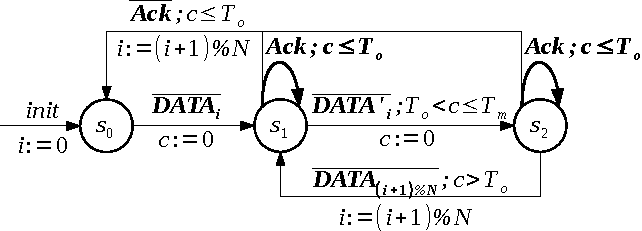
\includegraphics[width=0.7\textwidth]{./figures/dot11_tx_checker.pdf}
  \caption{\textbf{Augmented Monitor State Machine.} Augmented transitions are
  highlighted in bold face. $\overline{Pkt}$ means either $\epsilon$ or $Pkt$.}
  \label{fig:augment}
  \vspace*{-8mm}
\end{figure}

Before formally defining the augmented state machine, we first use an example to
illustrate the basic idea. Fig.~\ref{fig:augment} shows the augmented state
machine for 802.11 transmitter state machine shown in
Fig.~\ref{fig:dot11_tx_ta}.  For each existing transition (e.g., $s_0\rightarrow
s_1$), we add an \textit{empty transition} with same clock guards and resetting
clocks.  This accounts for the possibility when such packet was observed by
the DUT but missed by the sniffer.  Additionally, for each transition triggered
by a \textit{receiving} packet (i.e., $p.dest = DUT$), such as $s_1\rightarrow
s_0$ and $s_2\rightarrow s_0$, we add a \textit{self transition} with the same
trigger packet and clock guards, but an empty set of resetting clocks and no
assignments to variables. This allows the state machine to make progress when the sniffer missed such packets.

There are two things to note. First, self transitions are added only for
packets sent \textit{to} the DUT, since the sniffer will not overhear packets
\textit{from} the DUT if they were not sent by the DUT. Second, no augmented
transitions are added for the packets that are sent to DUT yet are missed by both
the DUT and the sniffer, since such packets do not cause difference between the
DUT and sniffer traces.

The augmented state machine in Fig.~\ref{fig:augment} will accept the sniffer
packet traces $Tr_1$ and $Tr_2$ shown in Fig.~\ref{fig:sniffer_in_middle}.  For
instance, one accepting transition sequence on sniffer trace $Tr_1$ is
$s_0\rightarrow s_1 \rightarrow_s s_1\rightarrow s_2 \rightarrow s_0$, and the
sequence for $Tr_2$ is $s_0 \rightarrow s_1 \rightarrow_e s_2 \rightarrow s_0$,
where $\rightarrow$ is the transition from the original state machine,
$\rightarrow_e$ and $\rightarrow_s$ are the augmented empty and self transitions
respectively.

We now formally define the augmented state machine.%
\vspace*{-1mm}
\begin{definition}
  An augmented state machine $S^+$ for a monitor state machine $S$ is a 7-tuple
  $\{\boldsymbol{\Sigma^+}, \mathbb{S}, \mathbb{X}, s_0, C, \boldsymbol{E^+},
  G\}$, where $\mathbb{S}, \mathbb{X}, s_0, C, G$ are the same as $S$.
  $\Sigma^+=\{\epsilon\} \cup \Sigma$ is the augmented input alphabet with the
  empty symbol, and $E^+ \supset E$ is the set of transitions, which includes:
  \vspace*{-1mm}
  \begin{itemize}
    \item $E$: existing transitions (\textbf{Type-0}) in $S$.
    \item $E^+_1$: empty transitions (\textbf{Type-1}) for transitions in $E$.
    \item $E^+_2$: self transitions \textbf{(Type-2)} for transitions
      triggered by receiving packets.
  \end{itemize}
\end{definition}

\begin{figure}[t!]
\begin{algorithm}[H]
  \caption{Obtain Augmented Transitions $E^+$ from $E$}
  \label{alg:augment}
  \begin{algorithmic}[1]
    \Function{augment}{$E$}
    \Let{$E^+$}{$\emptyset$}
    \ForAll{$\langle s_i, v_i, s_j, v_j, p, g, C'\rangle \in E$}
      \Let{$E^+$}{$E^+ \cup \{\langle s_i, v_i, s_j, v_j, p, g, C'\rangle\}$\Comment{Type-0}}
      \label{alg:augment:type0}
      \Let{$E^+$}{$E^+ \cup \{\langle s_i, v_i, s_j, v_j, \boldsymbol{\epsilon}, g, C'\rangle\}$\Comment{Type-1}}
      \label{alg:augment:type1}
      \If{$p.dest = DUT$}
      \Let{$E^+$}{$E^+ \cup \{\langle s_i, v_i, \boldsymbol{s_i},
      \boldsymbol{v_i}, p, g, \boldsymbol{\emptyset}\rangle\}$\Comment{Type-2}}
        \label{alg:augment:type2}
      \EndIf
    \EndFor
    \State \Return{$E^+$}
    \EndFunction
  \end{algorithmic}
\end{algorithm}
\vspace*{-12mm}
\end{figure}

Algorithm~\ref{alg:augment} describes the process of transforming $E$ into
$E^+$. In particular, Line~\ref{alg:augment:type0} adds existing transitions in
$E$ to $E^+$, while line~\ref{alg:augment:type1} and~\ref{alg:augment:type2} add
Type-1 and Type-2 transitions to $E^+$ respectively.  We have highlighted the
elements of the tuple that differ from the underlying Type-0 transition. Note
that in Type-2 transitions, both the state and the variables stay the same after
the transition.

With augmented state machine $S^+$, we can use Type-1 transitions to
non-deterministically infer packets missed by the sniffer, and use Type-2
transitions to consume extra packets captured by the sniffer but missed by the
DUT.

A accepting run of $S^+$ on sniffer trace $Tr$ yields a mutation trace $Tr'$
which represents one possibility of the DUT trace. Specifically, $Tr'$ can be
obtained by adding missing packets indicated by Type-1 transitions to $Tr$, and
removing extra packets indicated by Type-2 transitions from $Tr$

We show that the VALIDATION problem is equivalent to the
satisfiability problem of $Tr$ on $S^+$.

\begin{theorem}
  There exists a mutation trace $Tr' \in \mathcal{M}(Tr)$ that satisfies $S$ if
  and only if $Tr$ satisfies $S^+$.
 \label{the:equivalent}
\end{theorem}
\begin{proof}
  Assume $Tr$ satisfies $S^+$, and $P$ is a sequence of accepting transitions,
  we construct a mutation trace $Tr'$ using $P$ and show that $Tr'$ satisfies
  $S$.

  \sloppy{%
    Initially, let $Tr'=Tr$, then for each \textit{augmented} transition $\langle s_i,
  v_i, s_j, v_j, \sigma, g, C'\rangle \in P$:
  }
  \begin{itemize}
    \item If this is a Type-1 transition, add $(t, p)$ to $Tr'$, where $t$ is a
      timestamp that satisfies $g$ and $p$ is the missing packet.
    \item If this is a Type-2 transition, remove corresponding $(t, p)$ from
      $Tr'$.
  \end{itemize}
  It is obvious that $Tr'$ is a mutation trace of $Tr$, since only receiving
  packets are removed in the process.

  Now we show that there exists a accepting transition sequence $P'$ of $S^+$ on
  input $Tr'$ that does not contain augmented transitions.  In particular, $P'$
  can be obtained by substituting all Type-1 transitions with corresponding
  original transitions, and removing all Type-2 transition.  Since $P'$ does not
  contain augmented transitions, it is also an accepting transition sequence of
  $S$ on input $Tr'$, hence $Tr'$ satisfies $S$.

  On the other hand, assume $Tr' \in \mathcal{M}(Tr)$ and $Tr'$ satisfies $S$.
  Suppose $P'$ is the accepting transition sequences of $S$ on input $Tr'$.
  We first note that $P'$ is also the accepting transitions of $S^+$ on input
  $Tr'$, since $E \subset E^+$.

  We construct a accepting transition sequence $P$ of $S^+$ on input $Tr$ as
  follows.
  \begin{itemize}
    \item For each packet $p \in Tr' \setminus Tr$, substitute the transition
      $\langle s_i, v_i, s_j, v_j, p, g, C'\rangle$ with the corresponding Type-1
      transition $\langle s_i, v_i, s_j, v_j, \epsilon, g, C'\rangle$.
    \item For each transition $\langle s_i, v_i, s_j, v_j, \sigma, g, C'\rangle$
      followed by packet $p \in Tr\setminus Tr'$, add a Type-2 self
      transition $\langle s_j, v_j, s_j, v_j, p, g, \emptyset\rangle$. This is
      possible since $Tr'$ is a mutation trace of $Tr$, thus  for all $p \in Tr'
      \setminus Tr$, $p.src \ne DUT$.
  \end{itemize}
  Therefore, $Tr$ satisfies $S^+$.
\end{proof}

By Theorem~\ref{the:equivalent}, the inherent uncertainty of the sniffer traces
is explicitly represented by the augmented transitions, and can be
systematically explored using the well established theory of state machine.

\begin{comment}
One immediate observation can be drawn from Theorem~\ref{the:equivalent} by
contradiction.

\begin{corollary}
  If $S^+$ rejects $Tr$, then $S$ rejects $Tr_{DUT}$.
  \label{cor:false_pos}
\end{corollary}
In the context of validation where we raise a violation alarm when $S^+$
rejects $Tr$, Corollary~\ref{cor:false_pos} provides a {\it sufficient} condition for reporting incorrect traces. 
However, when $S^+$ accepts $Tr$, $S$ could still reject $Tr_{DUT}$.
In other words, the conclusion of the validation can either be \textit{definitely
wrong} or \textit{possibly correct}, but not \textit{definitely correct}.
This is the fundamental limitation caused by the uncertainty of sniffer traces.
\end{comment}
